% Julian Burger
% Bastian Uhlig
% David Koch

\documentclass[
	headings=optiontotocandhead,% Erweiterung für das optionale Argument der
	% Gliederungsbefehle aktiviert.
	oneside,
	numbers=noenddot,% Keine Punkte am Ende der Gliederungsnummern und davon
	% abgeleiteten Nummern
	toc=flat, %Flache TOC --- kann man anpassen (auskommentieren)
	10pt, % Schriftgröße
	parskip=full, % Abstand zwischen Absätzen (ganze Zeile)
	listof=totoc, % Verzeichnisse im Inhaltsverzeichnis aufführen
	listof=flat, % mehr Abstand für grosse Zahlen
	numbers=noenddot, % kein Punkt am Ende bei Nummern
	%%enlargefirstpage,% Gibt es bei scrartcl nicht!!!!
	bibliography=totoc, % Literaturverzeichnis im Inhaltsverzeichnis aufführen
	%index=totoc, % Index im Inhaltsverzeichnis aufführen
	%captions=tableheading, % Beschriftung von Tabellen für Ausgabe oberhalb
	% der Tabelle formatieren
	%draft % Status des Dokuments (final/draft) draft hinzufügen zum anziegen
	%%der zeilen ende
	a4paper,DIV=14,
	% captions=tablesignature,
]{scrartcl}
\usepackage{setspace}
\onehalfspacing

\setcounter{secnumdepth}{3}

\usepackage[T1]{fontenc}
\usepackage[utf8]{inputenc}

\usepackage[english, ngerman]{babel, varioref} % your native language must be the last one!!

\usepackage{lastpage}
\usepackage{listings}
\usepackage{blindtext}

\usepackage{tcolorbox}
\tcbuselibrary{skins}


%% Aufzählungen nicht so weit einrücken
\usepackage[inline]{enumitem}
%\setitemize{leftmargin=*}
% Listen etwas wenige einrücken, erfordert enumitem
\setitemize{labelindent=2em,labelsep=0.5cm,leftmargin=12ex}

\usepackage{lmodern}

\usepackage{xspace}

\usepackage{graphicx}
\graphicspath{ {../assets} {../assets/Ansuchen} }

%%? \usepackage{textcomp}
\usepackage[hyphens]{url}
\usepackage{makeidx}
\makeindex
%%? \usepackage{graphicx}
\usepackage[numbers]{natbib}
\PassOptionsToPackage{normalem}{ulem}
\usepackage{ulem}

\usepackage{needspace}

\setlength\partopsep{0.5ex}%schoenere Listen
\usepackage[bottom]{footmisc}%fussnote ganz unten

\usepackage[]{microtype}
\UseMicrotypeSet[protrusion]{basicmath} % disable protrusion for tt fonts

\usepackage{multirow}   % Allows table elements to span several rows.
\usepackage{booktabs}   % Improves the typesettings of tables.
\usepackage{subcaption} % Allows the use of subfigures and enables their referencing.
\usepackage[ruled,linesnumbered]{algorithm2e} % Enables the writing of pseudo code.
\usepackage[usenames,dvipsnames,table]{xcolor} % Allows the definition and use of colors. This package has to be included before tikz.
\usepackage{nag}       % Issues warnings when best practices in writing LaTeX documents are violated.
\usepackage{todonotes} % Provides tooltip-like todo notes.

\usepackage{color}
\usepackage[binary-units]{siunitx}

%% Override default figure placement To be within the flow of the text rather
%% than on it's own page.
\usepackage{float}
\usepackage{placeins}
% \makeatletter
% \def\fps@figure{H}
% \makeatother

%% bei vielen Bildern o.ä sinnvoll: Seite muss nicht bis ganz unten gefüllt werden
% \raggedbottom

%\usepackage{footbib} %  footcite, needs other tooling
%% for pandoc2 images
\makeatletter
\def\maxwidth{\ifdim\Gin@nat@width>\linewidth\linewidth\else\Gin@nat@width\fi}
\def\maxheight{\ifdim\Gin@nat@height>\textheight\textheight\else\Gin@nat@height\fi}
\makeatother
% Scale images if necessary, so that they will not overflow the page
% margins by default, and it is still possible to overwrite the defaults
% using explicit options in \includegraphics[width, height, ...]{}
\setkeys{Gin}{width=\maxwidth,height=\maxheight,keepaspectratio}

%% bessere Suche im PDF
\input{glyphtounicode}
\pdfgentounicode=1
%%%%%%%%%%%%%%%%%%%%%%%%%%%%%%%%%%%%%%%%%%%%%%%%%%%%%%%%%%%%%%%%%%%%%%%%%%%%%%%%%%

%  Kopf und Fußzeilen -- links und rechts verschieden
\newcommand{\kopfTXT}{\sffamily{\textbf{\small{HÖHERE TECHNISCHE BUNDESLEHRANSTALT Wien 3 Rennweg}}\\
Höhere Abteilung für Mechantronik \\
Höhere Abteilung für Informationstechnologie\\
Fachschule für Informationstechnik}}

\tcbset{headerBoxStyle/.style={
          enhanced, frame hidden, interior hidden, top=-0.15cm, bottom=-0.1cm, borderline west = {4pt}{0pt}{red}
}}
\newtcolorbox{headerBox}[1][]{headerBoxStyle, #1}

\newcommand{\kopfbild}{\voffset7mm
\includegraphics[width=50mm]{HTL3RLogo}}
\newcommand{\kopfHTL}{\begin{headerBox}
\kopfTXT
\end{headerBox}}

\usepackage[automark,footsepline,plainfootsepline]{scrlayer-scrpage}
\setkomafont{pageheadfoot}{\normalcolor\footnotesize\scshape}
\setkomafont{pagenumber}{\normalfont\normalsize}
\clearpairofpagestyles
\ihead{\headmark}
\ohead{\kopfbild}
\ihead{\kopfHTL}
\ifoot{\smaller{DA Ansuchen}}
\ofoot{Seite \pagemark/\pageref{LastPage}}
\ModifyLayer[addvoffset=-.6ex]{scrheadings.foot.above.line}% Linie verschieben
\ModifyLayer[addvoffset=-.6ex]{plain.scrheadings.foot.above.line}% Linie verschieben
\setlength{\headheight}{46pt}

% alle Seiten mit Kopfzeile
%\renewcommand{\chapterpagestyle}{scrheadings}

%% Code Beispiele
%% eine Variante
\usepackage{listings}
\renewcommand{\lstlistingname}{\inputencoding{utf8}Listing}

\usepackage{tabularx}
\usepackage{scrhack}

\usepackage{array}
\newcommand\Tstrut{\rule{0pt}{3.2ex}}         % = `top' strut
\newcommand\Bstrut{\rule[-1.5ex]{0pt}{0pt}}   % = `bottom' strut

\newenvironment{nstabbing}
	{\setlength{\topsep}{-\parskip}
		\setlength{\partopsep}{-\parskip}
		\tabbing}
	{\endtabbing}

\usepackage{titlesec}
% \titleformat{?Überschriftenklasse?}[Absatzformatierung?]{?Textformatierung?} {?Nummerierung?}{?Abstand zwischen Nummerierung und Überschriftentext?}{?Code vor der Überschrift?}[?Code nach der Überschrift?]
\titleformat{\section}[hang]{\Large\bfseries\sffamily}{\thesection\quad}{-1.2ex}{}
\titleformat{\subsection}[hang]{\large\bfseries\sffamily}{\thesubsection\quad}{-1.2ex}{}
\titleformat{\subsubsection}[hang]{\large\bfseries\sffamily}{\thesubsubsection\quad}{-1.2ex}{}
\titleformat{\paragraph}[hang]{\large\bfseries\sffamily}{\theparagraph\quad}{-1.2ex}{}

% \titlespacing{?Überschriftenklasse?}{?Linker Einzug?}{?Platz oberhalb?}{?Platz unterhalb?}[?rechter Einzug?]
\titlespacing{\section}{0pt}{6pt}{6pt}
\titlespacing{\subsection}{0pt}{6pt}{0pt}
\titlespacing{\subsubsection}{0pt}{6pt}{0pt}
\titlespacing{\paragraph}{0pt}{6pt}{0pt}

%% sollte das letzte Package sein
\usepackage[unicode=true,
bookmarks=true,bookmarksnumbered=false,bookmarksopen=false,
breaklinks=true,pdfborder={0 0 0},backref=false,colorlinks=false]
{hyperref}
\hypersetup{pdftitle={ITP-Vorlage},
	pdfauthor={Wer auch immer},
	pdfsubject={ITP},
	pdfkeywords={4CN, ITP}}
\urlstyle{same} % don't use monospace font for urls

% Auch Fußnoten bündig ausrichten
\deffootnote[]{1em}{1em}{\textsuperscript{\thefootnotemark\ }}
%% setup
\sloppy % weniger Meldungen
\voffset7mm % etwas nach unten

\newcommand{\fieldbox}[4]{%
  \begin{tikzpicture}
    \draw[fill=white] (0,0) rectangle (#1,#2);
    \node[text=gray, font=\small] at (#1/2,0.2) {#3};
    \node[text=black, font=\large] at (#1/2,#2/1.5) {#4};
  \end{tikzpicture}%
}

\renewcommand{\familydefault}{\sfdefault} % Dokument sans serif
%\renewcommand\tabularxcolumn[1]{m{#1}}
%\renewcommand{\tabularxcolumn}[1]{>{\small}m{#1}}

%%%%%%%%%%%%%%%%%%%%%%%%%%%%%%%%%%%%%%%%%%%%%%%%%%%%%%%%%%%%%%%%%%%%%%%%%%%%%%%%%%
\begin{document}
%% schöner: 10000 -- gar keine, 1000 als Mittelweg
\clubpenalty = 10000 % Schusterjungen verhindern
\widowpenalty = 10000 % Hurenkinder verhindern
\displaywidowpenalty = 10000

{{\LARGE{{Ansuchen um Zulassung zur Diplomarbeit}}}}\\
\vspace{4mm}\\
\fieldbox{3.25cm}{1cm}{\footnotesize{Maturajahrgang}}{\large{2025}}
\hfill
\fieldbox{6cm}{1cm}{\footnotesize{Projektnummer (durch AV vergeben)}}{\large{}}\\ \\
\begin{tikzpicture}
  \draw[fill=white] (0,0) rectangle (\textwidth,1.68);
  \node[text=gray, font=\footnotesize, anchor=west] at (0.1,0.2) {Projektthema (Arbeitstitel)};
  \node[text=black, font=\Large, anchor=west] at (0.1,1.68/1.7) {\textbf{Fenrir}};
\end{tikzpicture}


% Projektteam
\large{\textbf{Projektteam}}
\begin{table}[h]
\begin{tabularx} {\textwidth} {
	|>{\hsize=.364\hsize}X
	|>{\hsize=.094\hsize}X
	|>{\hsize=.173\hsize}X
	|>{\hsize=.369\hsize}X|
}

\hline
\rowcolor[HTML]{D9D9D9} 
\rule{0pt}{17pt}
\textbf{\normalsize{Schülerin/Schüler}} & \multicolumn{1}{c|}{\textbf{\normalsize{Klasse}}} & \multicolumn{1}{c|}{\textbf{\normalsize{\begin{tabular}[c]{@{}c@{}}Individuelle\\ Betreuung\end{tabular}}}} & \multicolumn{1}{c|}{\textbf{\normalsize{Unterschrift}}} \\ \hline
\rule{0pt}{28pt}	\large{\textbf{David Koch}}	&	\multicolumn{1}{c|}{\large{4CN}}	&	\multicolumn{1}{c|}{\large{SDO}}	&              \\

\rule{0pt}{11pt}\textcolor[HTML]{A6A6A6}{\footnotesize{Projektleiter}}	&	&	& \textcolor[HTML]{808080}{\footnotesize{Unterschrift Projektleiter}}	\\ \hline

\rule{0pt}{28pt}	\large{\textbf{Bastian Uhlig}}	&	\multicolumn{1}{c|}{\large{4CN}}	&	\multicolumn{1}{c|}{\large{KUS}}	&              \\

\rule{0pt}{11pt}\textcolor[HTML]{A6A6A6}{\footnotesize{Stellv. Projektleiter}}	&	&	& \textcolor[HTML]{808080}{\footnotesize{Unterschrift Stellv. Projektleiter}}	\\ \hline

\rule{0pt}{28pt}	\large{\textbf{Julian Burger}}	&	\multicolumn{1}{c|}{\large{4CN}}	&	\multicolumn{1}{c|}{\large{SDO}}	&              \\

\rule{0pt}{11pt}\textcolor[HTML]{A6A6A6}{\footnotesize{Projektmitarbeiter}}		&	&	& \textcolor[HTML]{808080}{\footnotesize{Unterschrift Projektmitarbeiter}}	\\ \hline

\rule{0pt}{28pt}	\large{\textbf{Gabriel Vogler}}	&	\multicolumn{1}{c|}{\large{4CN}}	&	\multicolumn{1}{c|}{\large{SDO}}	&              \\

\rule{0pt}{11pt}\textcolor[HTML]{A6A6A6}{\footnotesize{Projektmitarbeiter}}		&	&	& \textcolor[HTML]{808080}{\footnotesize{Unterschrift Projektmitarbeiter}}	\\ \hline
\end{tabularx}
\end{table}


\large{\textbf{Projektbetreuung:}}
\begin{table}[h]
\begin{tabularx} {\textwidth} {
	|>{\hsize=.462\hsize}X
	|>{\hsize=.538\hsize}X|
}

\hline
\rule{0pt}{28pt}	\large{\textbf{Christian Schöndorfer}}	&              \\
\rule{0pt}{11pt}\textcolor[HTML]{A6A6A6}{\footnotesize{Individuelle Betreuung (Hauptbetreuung)}}	&	\textcolor[HTML]{A6A6A6}{\footnotesize{Unterschrift Hauptbetreuer}}	\\ \hline
\rule{0pt}{28pt}	\large{\textbf{Clemens Kussbach}}	&              \\
\rule{0pt}{11pt}\textcolor[HTML]{A6A6A6}{\footnotesize{Individuelle Betreuung (Hauptbetreuung Stellv.)}}	&	\textcolor[HTML]{A6A6A6}{\footnotesize{Unterschrift Stellv. Hauptbetreuer}}	\\ \hline
\end{tabularx}
\end{table}


\large{\textbf{\textcolor[HTML]{A6A6A6}{Projektvergabe (durch AV):}}}

\begin{table}[h]
\begin{tabularx} {\textwidth} {
	|>{\hsize=.232\hsize}X
	|>{\hsize=.23\hsize}X
	|>{\hsize=.062\hsize}X
	|>{\hsize=.476\hsize}X|
}

\cline{1-2} \cline{4-4}
\rule{0pt}{17pt}\normalsize{\textcolor[HTML]{808080}{Hauptbetreuung:}}&&&\\ \cline{1-2}
\rule{0pt}{17pt}\normalsize{\textcolor[HTML]{808080}{HB Stellvertretung:}}&&&\\ \cline{1-2}
\rule{0pt}{17pt}\normalsize{\textcolor[HTML]{808080}{Indiv. Betreuungen:}}&&&\footnotesize{\textcolor[HTML]{808080}{Bewilligt (Unterschrift AV)}}\\ \cline{1-2} \cline{4-4}
\end{tabularx}
\end{table}

\newpage

\tableofcontents
\newpage

\section{Projektidee}

\subsection{Ausgangssituation}
Im Vergleich zur Cybersicherheit von IT-Systemen, die in letzten Jahrzehnten immense Fortschritte gemacht hat, ist die Absicherung von OT-Systemen bzw. sogenannten “Industrial Control Systems” (kurz ICS) vernachlässigt worden. Bis heute sind zahlreiche Betriebe weltweit vor äußeren Cyberangriffen auf ihre inneren Kontrollsysteme ungeschützt.
Die politische Lage der Welt spitzt sich zu, Angriffe auf kritische Infrastruktur nehmen zu. Immer mehr staatliche Akteure versuchen die kritischen Industrie- sowie Infrastrukturdienste ihrer Gegner anzugreifen und sind zu oft dabei erfolgreich, da die Absicherung des Übergangs zwischen IT- und OT-Netzwerken im Betrieb oftmals suboptimal ist. 
Die Diplomarbeit Fenrir zielt darauf ab, ein realitätsgetreues Netzwerk, inklusive IT- sowie OT-Bereich, wie es in der Industrie üblich wäre nachzubauen, anzugreifen und daraufhin gegen Angriffe zu härten. Dieser Prozess wird dokumentiert, um allen Projektmitarbeitern einen Einblick in den Berufsalltag von ICS-Security-Experten zu geben und somit auch für die derzeitige sowie zukünftige Arbeitswelt wertvolle Berufserfahrung zu sammeln.

\subsection{Beschreibung der Idee}
„Wie sichert man den Übergang zwischen IT und OT ausreichend vor Angriffen ab?“
Es wird eine physische Topologie gebaut, welche ein realitätsgetreues Heimnetz, inklusive IT- (Ac-tive Directory Büro- bzw. Serverumgebung) sowie OT-Bereich (Bus-Steuerungstechnik, die anzusteuernden Aktoren/Sensoren, SCADA-System), repräsentieren soll.
Der OT-Bereich besteht aus einem von Herr Prof. Schöndorfer bereitgestellten Bewässerungssystem. Dies setzt sich unter anderem aus Gartenbrunnen, Wassertanks und Pumpen zusammen, wo-bei diese Gegenstände mit verbauter Aktorik und/oder Sensorik als Ansteuerungsziel einer SPS gelten. Diese wird später auch als Angriffsziel verwendet, wobei ein Angreifer beispielsweise das Bewässerungssystem komplett lahmlegen, oder auch mit der Manipulation dessen einen Wasserschaden verursachen könnte.
Als Ziel des Projektes gilt nicht nur ein vor äußeren sowie inneren Cyberangriffen abgesichertes Netzwerk aufzustellen, sondern auch eine für Interessenten (d.h. mögliche Firmenpartner) wiederverwertbare Dokumentation des Konfigurations- bzw. Absicherungsprozesses, etwa im Stil eines Handbuchs.
Um diesen Absicherungsprozess dokumentieren zu können, braucht es zuerst ein ungesichertes Netz, auf welchem ohne weitere Beschränkungen Hackerangriffe stattfinden können. Dieses wird darauf mit SOTA\footnote{State of the Art}-Tools abgesichert, um äußere Angriffe zu verhindern. Das heißt, dass die Projektumsetzung in zwei Phasen stattfinden wird:

\begin{enumerate}
\item \underline{Umsetzung eines realitätsgetreuen, ungesicherten Netzwerks:}\\
Durch absichtliche Fehlkonfiguration der Firewalls sowie mangelnder Netzwerksegmentierung können IT-Hosts sehr einfach auf betriebskritische OT-Komponenten zugreifen bzw. diese lahmlegen. Es werden auf dieses ungesicherte Netzwerk vom Projektteam für den Zweck selbst programmierte Malware, aber auch aus echten Cyberangriffen gesammelte Netzwerkwürmer eingesetzt (Diese werden von der Ikarus Security Software GmbH bereit-gestellt). Mithilfe von Sniffing-Tools sowie der Nozomi Guardian wird der Angriffsverlauf überwacht sowie aufgezeichnet und anschließend werden die ausgenutzten Schwachstellen dokumentiert, um diese in der 2. Phase der Diplomarbeit gezielt beheben zu können.

\item \underline{Umsetzung eines realitätsgetreuen, gesicherten Netzwerks:}\\
Zur Abgrenzung zwischen IT und OT wird eine FortiGate-Firewall mit strikter Netzwerkzugangskontrollkonfiguration verwendet, um unter anderem eine Zugriffskontrolle auf das OT-Netz zu etablieren, aber auch die Integration einer Nozomi Guardian zur OT-Netzwerküberwachung zu ermöglichen. Diese Nozomi Guardian liest aktiv über ein SPAN-Mirroring jeglichen Traffic innerhalb des gesamten OT-Netzwerks mit, um Angriffe sowie Fehlkonfiguration für einen Netzwerkadministrator stets leicht ersichtlich zu machen.

\end{enumerate}
Als Busprotokoll wird voraussichtlich Modbus eingesetzt, außerdem wird dieses im OT-Bereich – soweit es geht – TCP/IP-enkapsuliert, das heißt, dass die speicherprogrammierbaren Steuerungen über einen Ethernet-Anschluss verfügen müssen. Erst auf der „last mile“ zu der Aktorik bzw. Sensorik wird serielle Verkabelung eingesetzt.

\newpage
Die gesamte Netzwerktopologie der Diplomarbeit sieht vereinfacht im Purdue-Modell wie folgt aus:
\todo{AAAAAAA}
\begin{figure}[h]
	\centering
	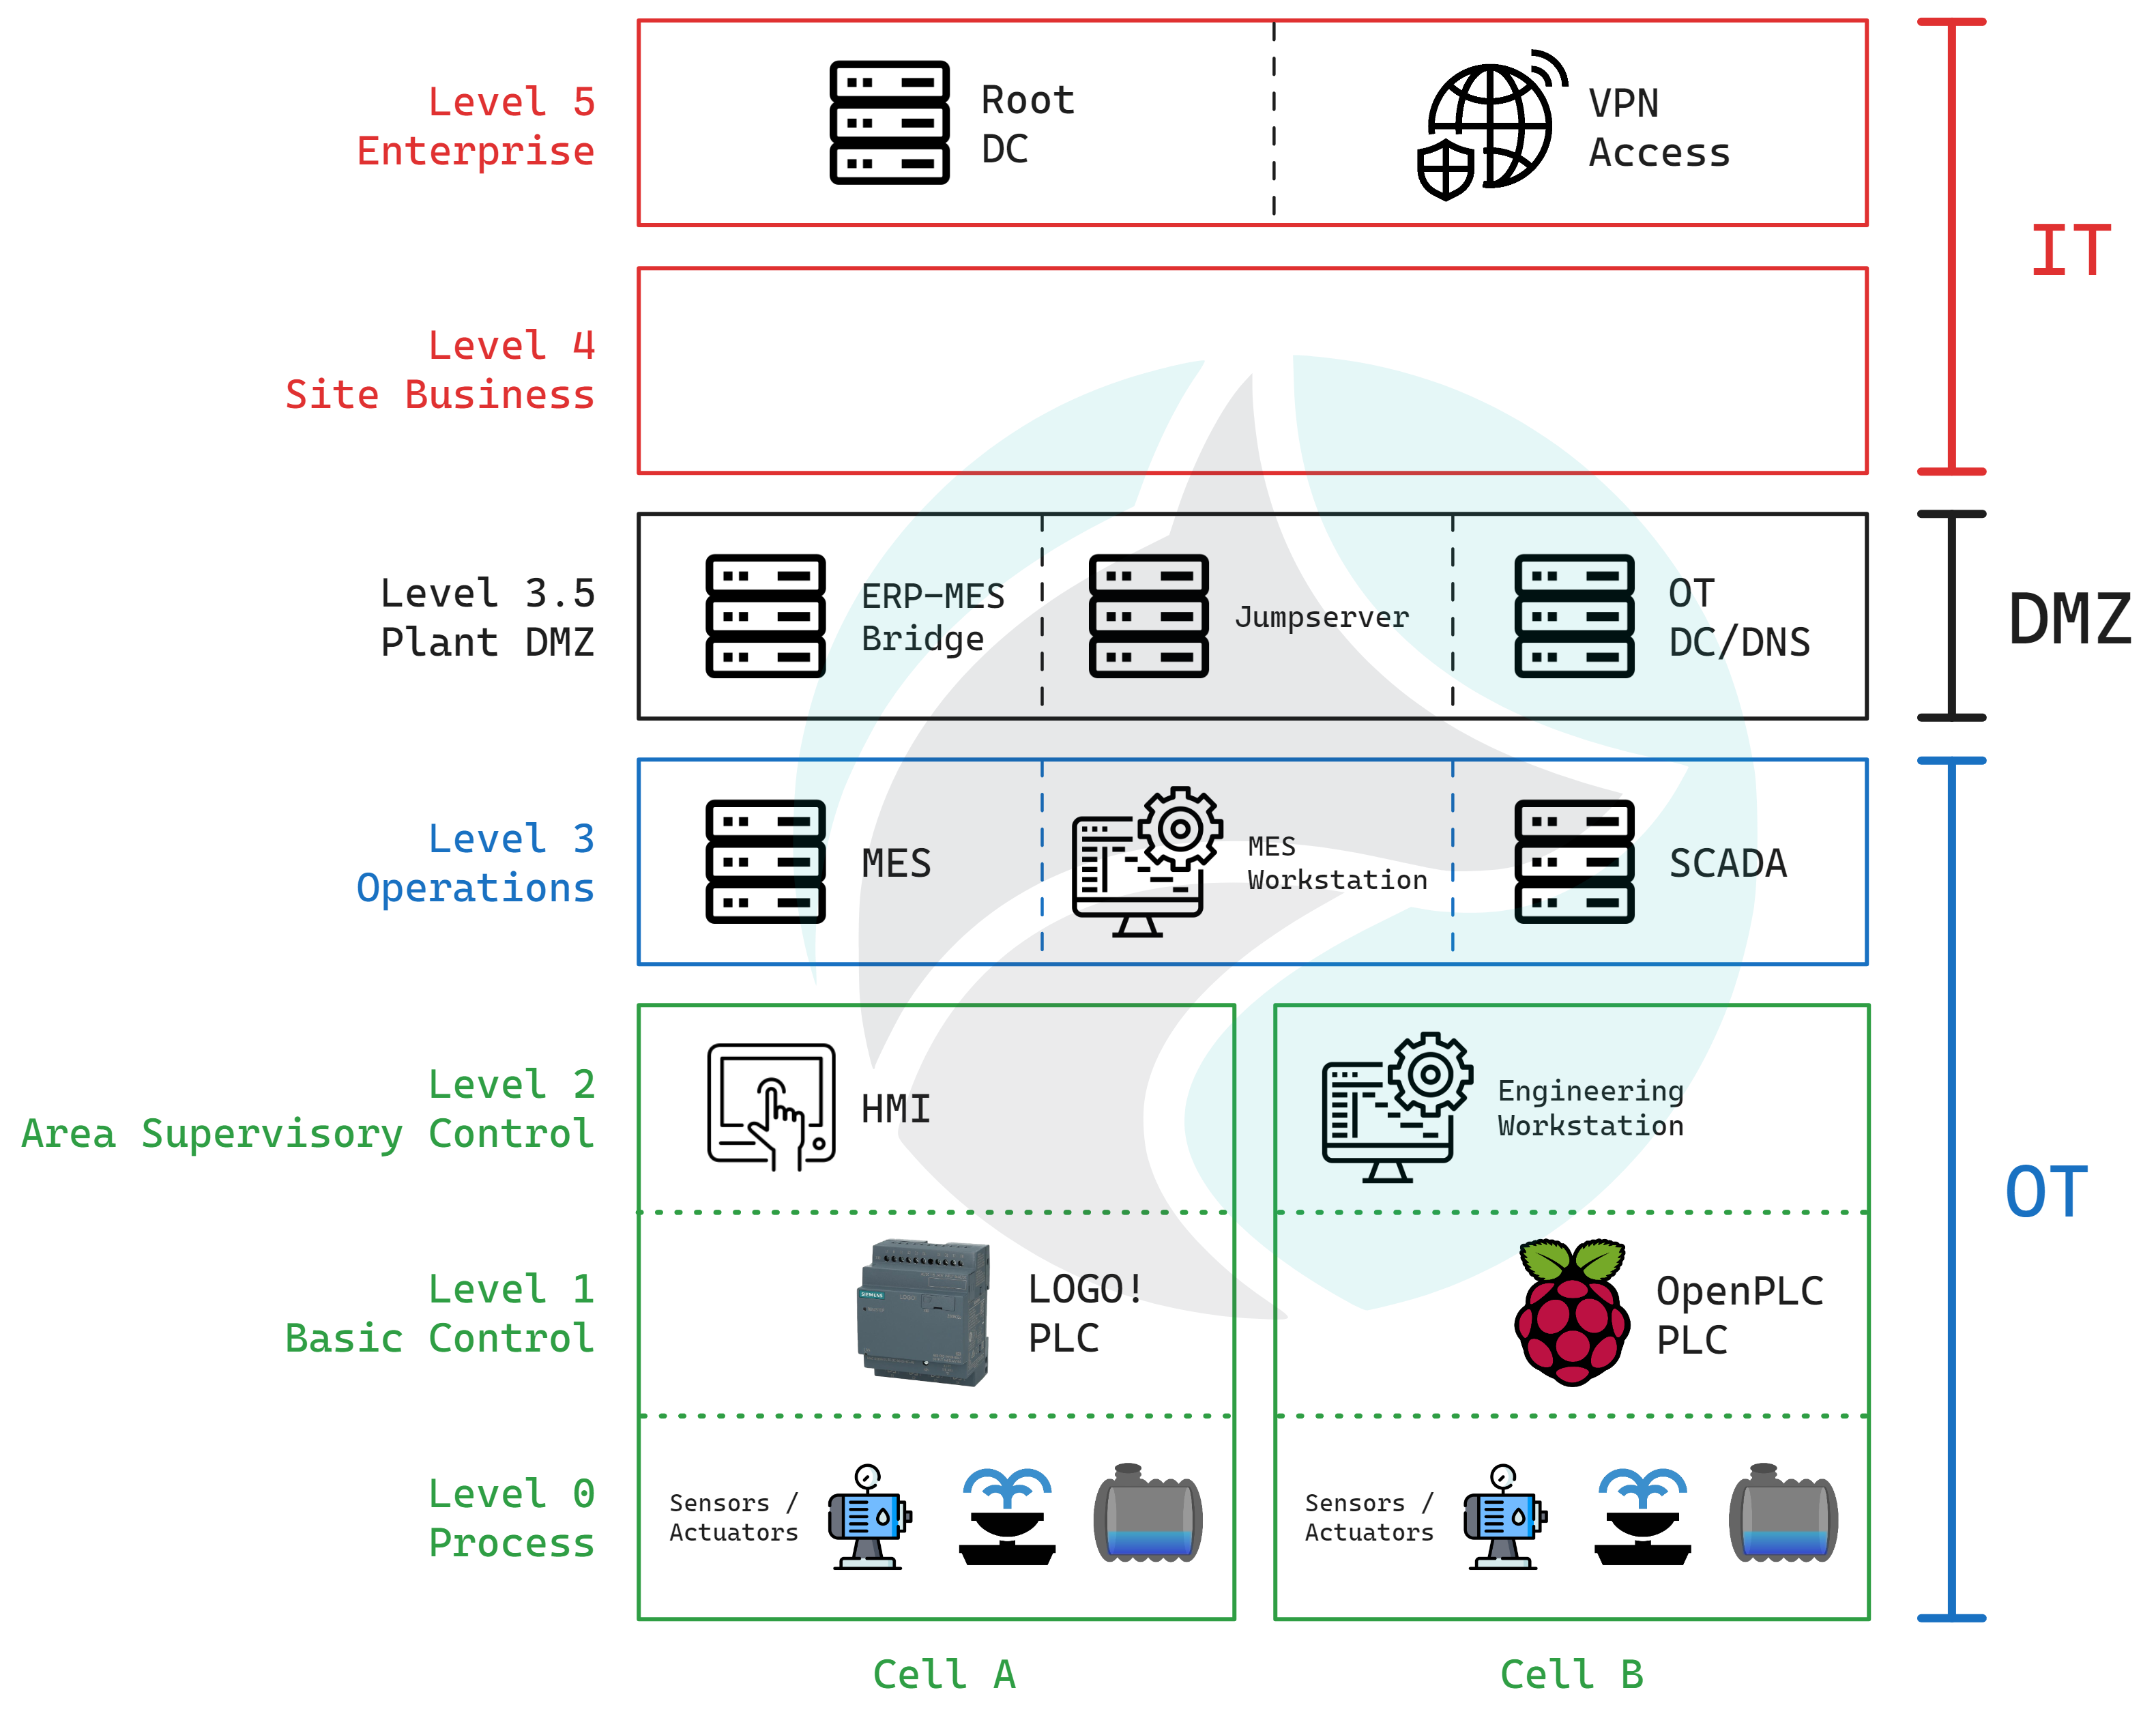
\includegraphics[width=1\linewidth]{Purdue}
	\caption[]{Vereinfachte Topologie der Diplomarbeit Fenrir im Purdue-Modell}
\end{figure}
\FloatBarrier 

\newpage
\section{Projektziele}
\subsection{Hauptziele}
\begin{enumerate}[start=1,label={\bfseries Ziel-H \arabic*},leftmargin=*,wide]
\item{\bfseries{Ungesicherte Netzwerktopologie}}\\
Die gesamte Netzwerktopologie ist umgesetzt und funktioniert einwandfrei, jedoch mit fehlender Absicherung vor äußeren Angriffen.
\begin{enumerate}[label=\alph*.]
\item{\underline{Planung der Topologie}}\\
Die gesamte Projekttopologie ist finalisiert und grafisch dargestellt.

\item{\underline{OT-Aufbau/Verkabelung}}\\
Der gesamte OT-Bereich ist fertig aufgebaut und verkabelt.

\item{\underline{IT-Aufbau/Verkabelung}}\\
Der gesamte IT-Bereich läuft virtualisiert auf einer ESXi-Maschine und ist fertig verkabelt.

\item{\underline{Übergang \& DMZ IT/OT}}\\
Der IT- und der OT-Bereich sind zusammengeschlossen mittels einer FortiGate-FW. Diese lässt jeglichen Traffic zwischen IT und OT durchfließen und die DMZ bleibt vorerst ungenutzt.

\item{\underline{PLC-Programmierung}}\\
Alle SPSen im OT-Bereich sind je nach ihrem Zweck und der anzusteuernden Aktorik/Sensorik fertig programmiert.

\begin{enumerate}[label=\roman*.]
\item{\underline{Simatic}}\\
Die Siemens Simatic SPS wurde je nach Zweck mittels Siemens STEP 7 programmiert.

\item{\underline{LOGO!}}\\
Die Siemens LOGO! SPS wurde je nach Zweck mittels Siemens Comfort programmiert.

\item{\underline{OpenPLC}}\\
Die OpenPLC SPS, die auf einem Raspberry Pi 3b läuft, wurde je nach Zweck mittels des OpenPLC-Editors programmiert.
\end{enumerate}

\item{\underline{SCADA Aufsetzung}}\\
Das SCADA-System für die Überwachung des Betriebsprozesses im OT-Bereich ist fertiggestellt.

\begin{enumerate}[label=\roman*.]
\item{\underline{Konfiguration/Scripting}}\\
Die Aktoren und Sensoren der jeweiligen Betriebszellen sind im SCADA eingetragen und können erfolgreich ein- und ausgeschalten werden.

\item{\underline{Design}}\\
Die miteinander zusammenhängenden Aktoren und Sensoren der jeweiligen Betriebszellen sind im SCADA grafisch realitätsnah abgebildet.
\end{enumerate}

\item{\underline{HMI-Konfiguration}}\\
Alle HMI-Geräte sind ihrem Zweck nach konfiguriert worden, um den Betriebsprozess überwachen zu können.

\item{\underline{Engineer-Workstation}}\\
Die Ubuntu-Workstation zum Programmieren von der SPSen ist fertig aufgesetzt und hat die Programme Siemens STEP 7, Siemens Comfort und OpenPLC-Editor installiert.

\item{\underline{AD-Umgebung erstellt}}\\
Mithilfe von Active Directory ist ein Firmennetzwerk eines KMUs nachgebaut. Dieses trägt den Domänennamen htl3r.fenrir.com.

\begin{enumerate}[label=\roman*.]
\item{\underline{DC-Konfiguration}}\\
In der Active Directory Umgebung existieren zwei Domain Controller, welche untereinander redundant und somit ausfallsicher betrieben werden. Die FSMO-Rollen sind so gleichmäßig es geht auf diesen aufgeteilt, dazu sind beide für Optimierungszwecke ein Global Catalog-Server. Auch automatisierte tägliche Backups der AD-Datenbank und der Systemzustandsdateien beider Domain Controller finden statt und werden auf einem extra für Backups konzipierten File-Server (siehe "'Server konfiguriert"') gespeichert.
\item{\underline{OU-Struktur}}\\
Die einzelnen Objekte wie Computer sowie User der Active Directory Umgebung sind nach dem Business-Unit-Modell hierarchisch in Organisational Units (kurz OUs) unterteilt und somit auch strukturiert.
\item{\underline{Konten/Gruppen-Erstellung \& Konfiguration}}\\
Die Benutzerkonten, Sicherheitsgruppen für Zugriffsrechte sowie Gruppenrichtlinien auf Assets innerhalb des Netzwerks sind erstellt.
\item{\underline{Prometheus Monitoring?}}\\
Ein Ubuntu-Server mit einer Prometheus-Konfiguration steht im IT-Netzwerk und überwacht die AD-Domain-Controller. Unter anderem werden Systemressourcen, Datenverkehr sowie andere Teile der ADDS überwacht und auf einem Grafana Dashboard dargestellt.
\end{enumerate}

\item{\underline{Endgeräte konfiguriert}}\\
Endgeräte, die oftmals in Büroumgebungen aufzufinden sind wie Office-PCs, Laptops, Drucker sind Teil des IT-Netzwerks und sind in der Active Directory Umgebung integriert.

\item{\underline{Server konfiguriert}}\\
Ein Mail-Server, auf welchem Microsoft Exchange läuft, und ein File-Server, welcher zur Speicherung von Backups sowie für das Hosting von Shares zuständig ist sind beide im IT-Netzwerk und somit auch in der Active Directory Umgebung integriert.

\end{enumerate}
\item{\bfseries{Gesicherte Netzwerktopologie}}\\
Alle Bereiche der Netzwerktopologie sind nach den unten angeführten Sicherheitskriterien gehärtet. Die Topologie gilt nun als industriegemäß/realitätsgetreu sicher vor äußeren Angriffen.

\begin{enumerate}[label=\alph*.]
\item{\underline{Firewall Konfiguration}}\\
Alle Firewalls innerhalb der Topologie wurden nach den angegebene Sicherheitskriterien konfiguriert. 

\begin{enumerate}[label=\roman*.]
\item{\underline{Uplink}}\\
An der Schnittstelle zwischen dem IT-Netzwerk dieser Diplomarbeit und der Anbindung an den ISP der HTL Rennweg steht eine FortiGate-60F Firewall. Diese schützt unter anderem vor äußeren Angriffen auf das Netzwerk und betreibt Traffic-Shaping sowie Data Loss Prevention (kurz DLP) der Datenpakete des IT-Netzwerks. Um dies zu ermöglichen wird mittels Deep Packet Inspection (kurz DPI) so gut wie jedes einzelne Datenpaket analysiert und auf Zweck sowie mögliche Schädlichkeit überprüft.

\item{\underline{Übergang IT/OT}}\\
Der Übergang zwischen der OT- und der IT-Welt ist mittels einer FortiGate-60F Firewall so abgesichert, dass nur die berechtigte Workstation in das OT-Netzwerk eingreifen kann, und auch dort nur auf das SCADA-System bzw. die SPS-Workstation.

\item{\underline{OT-Zellen}}\\
Innerhalb des OT-Netzwerks unterteilen schienen-montierte FortiGateRugged-60F Firewalls manche Bereiche in sogenannte OT-Zellen.
\end{enumerate}

\item{\underline{Jump Server}}\\
Der Jump Server für den VPN-Zugriff vom IT-Netzwerk in das OT-Netzwerk ist fertig aufgesetzt und liegt in der DMZ der Übergangs-Firewall.

\item{\underline{OT-Segmentierung}}\\
Das OT-Netzwerk wurde in Zellen mit einer Firewall pro Zelle als Abgrenzung segmentiert, um die Betriebssicherheit zu erhöhen.

\item{\underline{Nozomi Guardian}}\\
% sowie an der Uplink-FW ist maybe fuisch who knows
Eine Nozomi Guardian ist in der Netzwerktopologie vertreten, um den Datenverkehr, der hauptsächlich im OT-Netzwerk stattfindet, zu überwachen.
\begin{enumerate}[label=\roman*.]
\item{\underline{Installation}}\
Eine virtualisierte Ubuntu-Installation mit den von der Ikarus vorinstallierten 	Guardian Servers läuft auf einer ESXi-Maschine.

\item{\underline{Einbindung}}\\
Eine Nozomi Guardian ist an der Übergangs-Firewall (sowie an der Uplink-FW?) angeschlossen und erhält über RSPAN-Mirroring Traffic vom OT- sowie dem IT-Netzwerk. Sie wertet diesen Traffic schließlich aus und stellt diesen für Netzwerkadministrator*innen leicht ersichtlich dar.
\end{enumerate}
\end{enumerate}

\item{\bfseries{Absicherungshandbuch}}\\
Der Prozess des Aufbaus sowie der Absicherung der Topologie sind in einem Handbuch aufgefasst. Dieses ist mittels \LaTeX geschrieben und dient als Nachschlagewerk für angehende OT-Security-Spezialisten. Unter anderem werden im Handbuch folgende Punkte festgelegt:
\begin{enumerate}[label=\alph*.]
\item{\underline{Wireshark Überwachung}}\\
Es ist über ein Throwing Star LAN Tap der Datenverkehr zwischen den Geräten im IT- sowie dem OT-Netzwerk stichprobenartig mittels Wireshark mitgelesen. Der aufgezeichnete Da-tenverkehr wurde darauf auf die laufenden Kommunikationsprozesse analysiert/dokumentiert.

\item{\underline{Nozomi Guardian Überwachung}}\\
Es ist mittels der Nozomi Guardian der Datenverkehr zwischen den Geräten im IT- sowie dem OT-Netzwerk stichprobenartig mitgelesen. Der aufgezeichnete Datenverkehr wurde darauf auf die laufenden Kommunikationsprozesse analysiert/dokumentiert.

\item{\underline{Handbuch erstellt}}\\
Die Ergebnisse/Erkenntnisse der Diplomarbeit sind in einem Absicherungshandbuch zusammengeschrieben. Dieses inkludiert unter anderem Abschnitte zum Aufbau der Topologie, zur Theorie hinter der OT-Absicherung, zur Absicherung der Topologie und zum aufgekommenen Datenverkehr innerhalb der Topologie.
\end{enumerate}
\end{enumerate}

\subsection{Optionale Ziele}
\begin{enumerate}[start=1,label={\bfseries Ziel-O \arabic*},leftmargin=*,wide]
\item{\bfseries{FCP Network Security Zertifizierung}}\\
Alle Projektteammitglieder haben zum Zeitpunkt der Abgabe der Diplomarbeit die von Fortinet bereitgestellte FCP Network Security Zertifizierung erfolgreich erworben.

\item{\bfseries{Medienauftritt}}\\
Für die Repräsentation des Projektteams aber auch der während der Diplomarbeit erledigten Arbeit sind verschiedene Medienauftritte angelegt worden.

\begin{enumerate}[label=\roman*.]
\item{\underline{Social Media}}\\
Es ist ein Social-Media-Konto auf Instagram namens fenrir.ot angelegt worden. Auf diesem Konto werden die Projektteammitglieder und die Diplomarbeitsidee der Öffentlichkeit vorgestellt. Dazu wird der Arbeitsablauf während des Diplomarbeitsverlaufs mittels Fotos dokumentiert und dort hochgeladen.

\item{\underline{Website}}\\
Unter der von easyname gehosteten URL fenrir-ot.at ist eine dem Projekt-Styleguide nach erstellten Website abrufbar. Auf dieser werden die Projektteammitglieder und die Diplomarbeitsidee der Öffentlichkeit vorgestellt.
\end{enumerate}

\item{\bfseries{Sticker drucken}}\\
Es sind Sticker mit dem Fenrir Logo gedruckt und an Interessierte vergeben.
\end{enumerate}

\subsection{NICHT Ziele}
\begin{enumerate}[start=1,label={\bfseries Ziel-N \arabic*},leftmargin=*,wide]
\item{\bfseries{Topologie Aufbau}}\\
Das Projektteam ist für den Abbau der gesamten Netzwerktopologie nach Abschluss der Diplomarbeit zuständig.
\item{\bfseries{Endpoint-Security}}\\
Auf den Endgeräten im IT-Netzwerk (PC-Hosts z.B.) ist eine Art von Endpoint-Security installiert (SentinelOne z.B.)
\end{enumerate}
\newpage

\subsection{Individuelle Aufgabenstellungen der Teammitglieder im Projekt}
\begin{table}[h]
	\begin{tabularx} {\textwidth} {
			|>{\hsize=.75\hsize}X
			|>{\hsize=.25\hsize}X
		}
		
		\hline
		\rowcolor[HTML]{D9D9D9} 
		\rule{0pt}{15pt}
		\textbf{\normalsize{David Koch}} & \multicolumn{1}{c|}{\textbf{\normalsize{Projektleiter}}} \\ \hline
		
		\rule{0pt}{20pt} LOREM IPSUM \\
		\rule{0pt}{11pt}\textcolor[HTML]{A6A6A6}{\footnotesize{Themenschwerpunkt}} \\ \hline
		
		\begin{itemize}[itemsep=0pt, parsep=0pt, topsep=0pt]
			\item{Fortinet}
			\item{Ikarus Security Software GmbH}
		\end{itemize}
		
		\rule{0pt}{11pt}\textcolor[HTML]{A6A6A6}{\footnotesize{Aufgabenstellung}} \\ \hline
	\end{tabularx}
\end{table}

\begin{table}[h]
	\begin{tabularx} {\textwidth} {
			|>{\hsize=.7\hsize}X
			|>{\hsize=.3\hsize}X
		}
		
		\hline
		\rowcolor[HTML]{D9D9D9} 
		\rule{0pt}{17pt}
		\textbf{\normalsize{David Koch}} & \multicolumn{1}{c|}{\textbf{\normalsize{Projektleiter}}} \\ \hline
		
		LOREM IPSUM \\
		\rule{0pt}{11pt}\textcolor[HTML]{A6A6A6}{\footnotesize{Themenschwerpunkt}} \\ \hline
		
		\begin{itemize}
			\item{Fortinet}
			\item{Ikarus Security Software GmbH}
		\end{itemize}
		
		\rule{0pt}{11pt}\textcolor[HTML]{A6A6A6}{\footnotesize{Aufgabenstellung}} \\ \hline
	\end{tabularx}
\end{table}

\newpage
\section{Projektorganisation}
\subsection{Grafische Darstellung}

\begin{figure}[h]
	\centering
	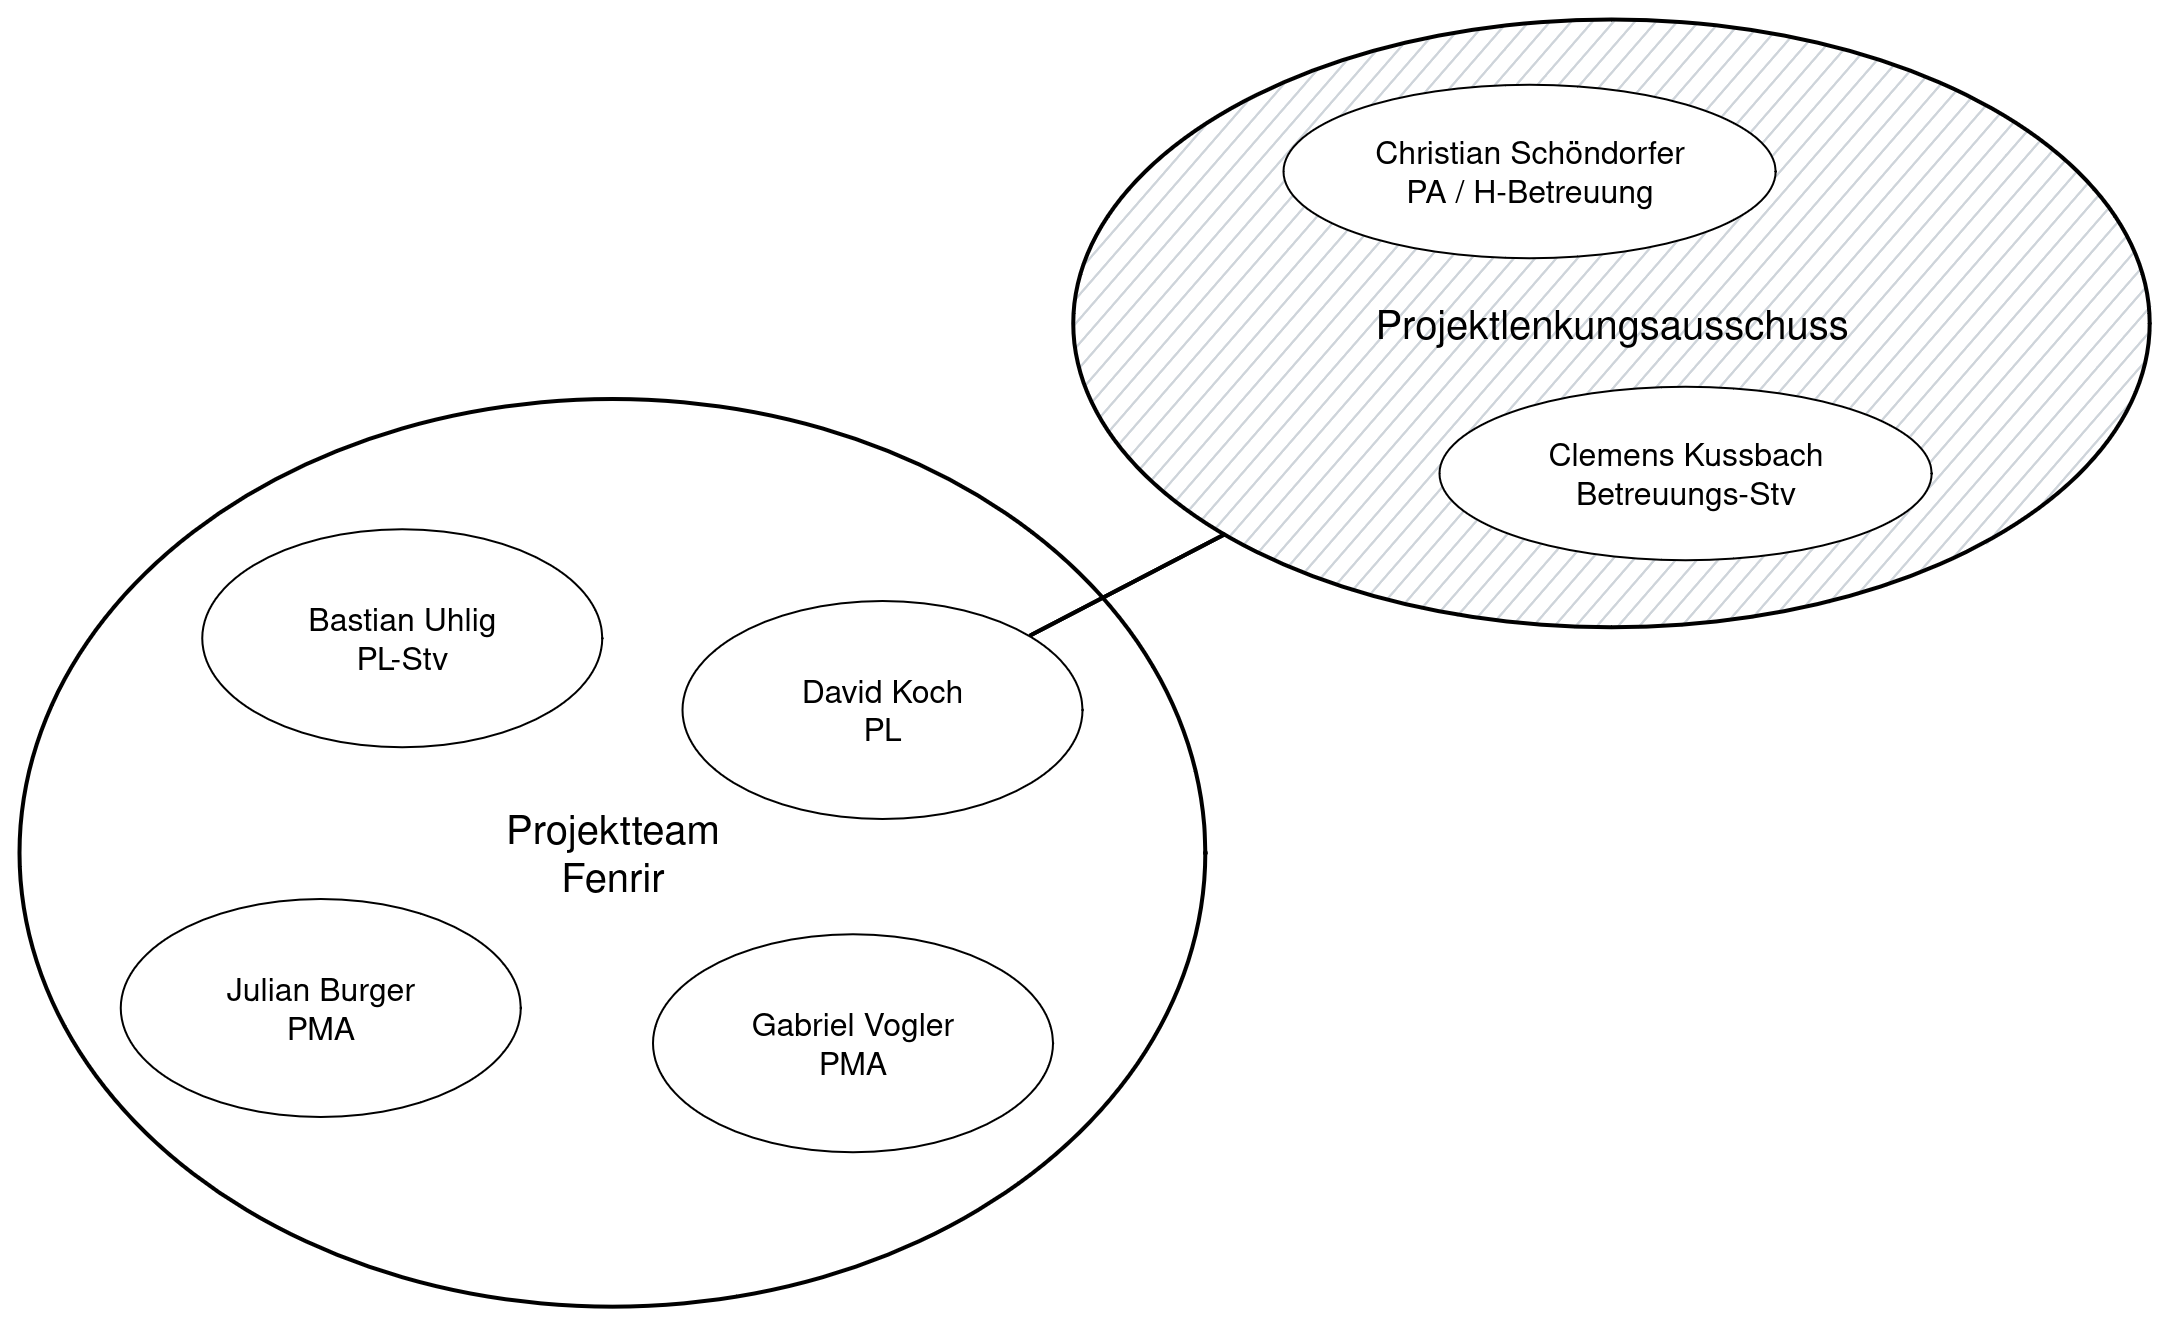
\includegraphics[width=1\linewidth]{Organigramm}
	\caption[]{Projektorganigramm der Diplomarbeit Fenrir}
\end{figure}
\FloatBarrier 

{\small\begin{spacing}{1.125}
Legende: \\
PA = Projektauftraggeber \\
PL = Projektleiter \\
PL-Stv = Projektleiter Stellvertretung \\
PMA = Projektmitarbeiter \\
H-Betreuung = Hauptbetreuung \\
Betreuung-Stv = Betreuung Stellvertretung \\
\end{spacing}}
\subsection{Projektteam}

\newpage
\section{Betrachtungsplan}

\begin{figure}[h]
	\centering
	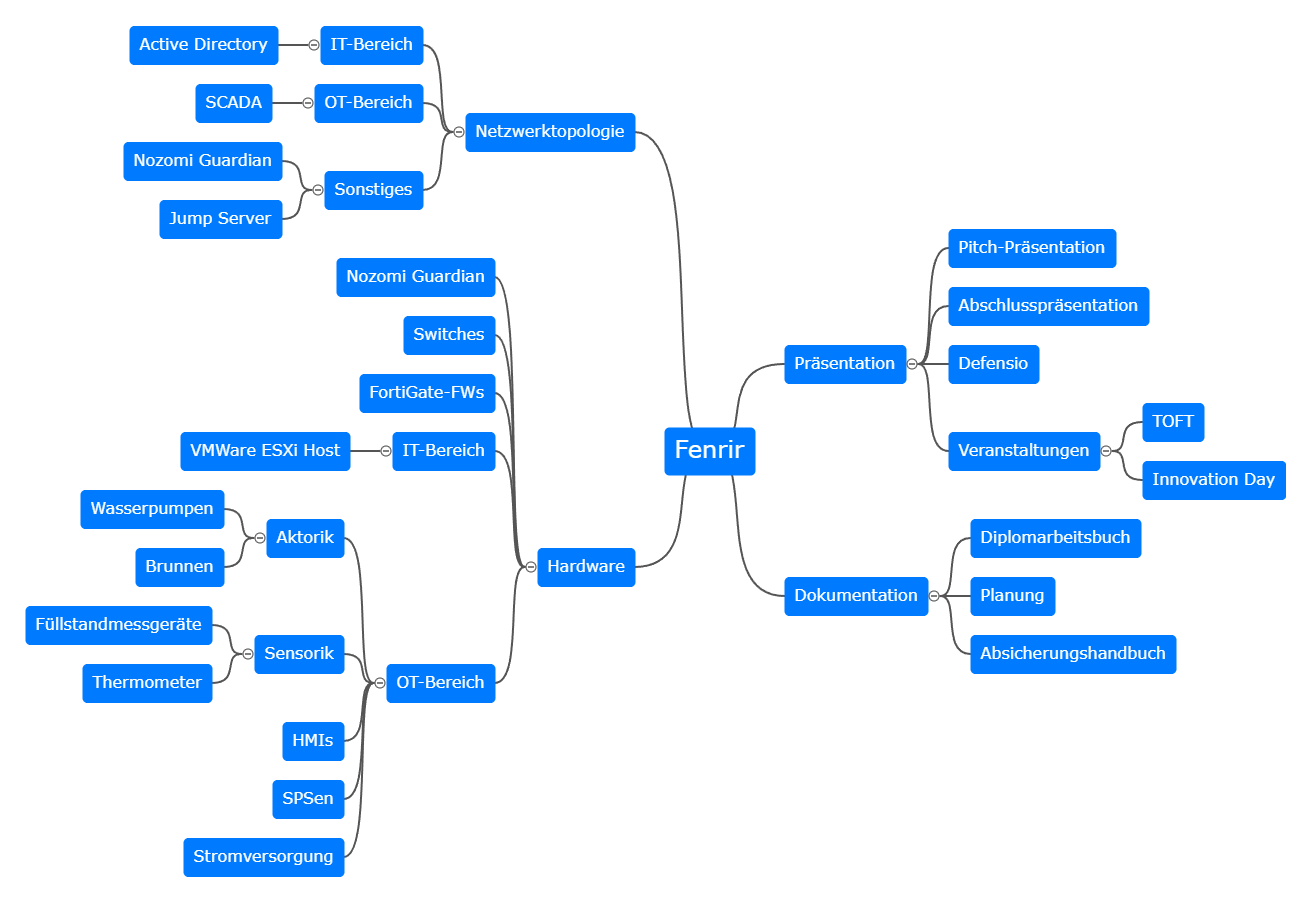
\includegraphics[width=1\linewidth]{Mindmap}
	\caption[]{Betrachtungsplan der Diplomarbeit Fenrir dargestellt als Mindmap}
\end{figure}
\FloatBarrier 

\newpage
\section{Budget}
\subsection{Erwartete Kosten für die Durchführung des Projektes}
\subsection{Kostendeckung}

\newpage
\section{Geplante externe Kooperationspartner}
Folgende Firmen liegen als geplante externe Kooperationspartner vor:
\begin{itemize}
	\item{Fortinet}
	\item{Ikarus Security Software GmbH}
\end{itemize}
Die Fortinet trägt zur Bereitstellung der Lizenzen für die in der Netzwerktopologie vorhandenen FortiGate-Firewalls sowie FortiSwitches bei.

Von der Ikarus Security Software GmbH wird ein Docker-Container, der eine Nozomi Guardian als Software innehält, sowie die für die Nozomi Guardian zugehörigen Lizenzen bereitgestellt. Dazu dient Herbert Dirnberger mit seiner Position von Industrial Cyber Security Expert als Berater im Bereich Absicherung des OT-Netzwerks.

\newpage
\section{Geplante Verwertung der Ergebnisse}
Nach Abschluss der Diplomarbeit bleibt nur das während der Arbeit erstellte Handbuch über, die gesamte Netzwerktopologie bleibt im Serverraum 078 bestehen und kann jederzeit abgebaut werden und die einzelnen Komponenten an den ursprünglichen Besitzer übergeben, das heißt, dass Herr Prof. Schöndorfer die von ihm geliehene Sensorik sowie Aktorik zurückbekommt, die von zuvorigen Diplomarbeiten wiederverwerteten Bauteile sowie mit schulischen Förderungsgeldern gekaufte Komponente werden an die HTL Rennweg übergeben und alle von den Projektmitglieder privat gekauften Bauteile gehen wieder in ihren Besitz über. 

\end{document}
